\chapter{相关理论与技术}\label{chap:theories_tech}

\section{Linux调度子系统}

% 内核Core调度流程
% 影响内核调度的关键因素
% - HZ
% - 调度类/机制
% - 调度策略/算法
% - 高质量的操作系统组件,如调度器,则可能需要数十年的时间来完善\citep{agache2020firecracker}

调度子系统是Linux内核的一个重要组成部分,其主要负责在多任务场景下,为系统中的每个进程分配CPU资源。Linux调度子系统通常可分为三层,各层为更上层提供了基本机制,各层的协作为复杂的调度机制的实现提供了可能,如图~\ref{fig:sched_arch}所示,位于最底层的Core调度机制提供了最基本的调度实现,包括抢占调度与非抢占调度,调度类层则针对不同调度目标,提供了包括实时调度、公平调度等特性,并且不同的调度类间存在优先级差异,最上层的调度策略则考虑到不同任务的差异,允许在调度类的基础之上,进一步划分任务的优先级,如在公平调度类中,就区分了NORMAL与BATCH类型的调度策略,同时也提供了系统调用来更灵活地设置任务静态优先级。

\begin{figure}[!htbp]
    \centering
    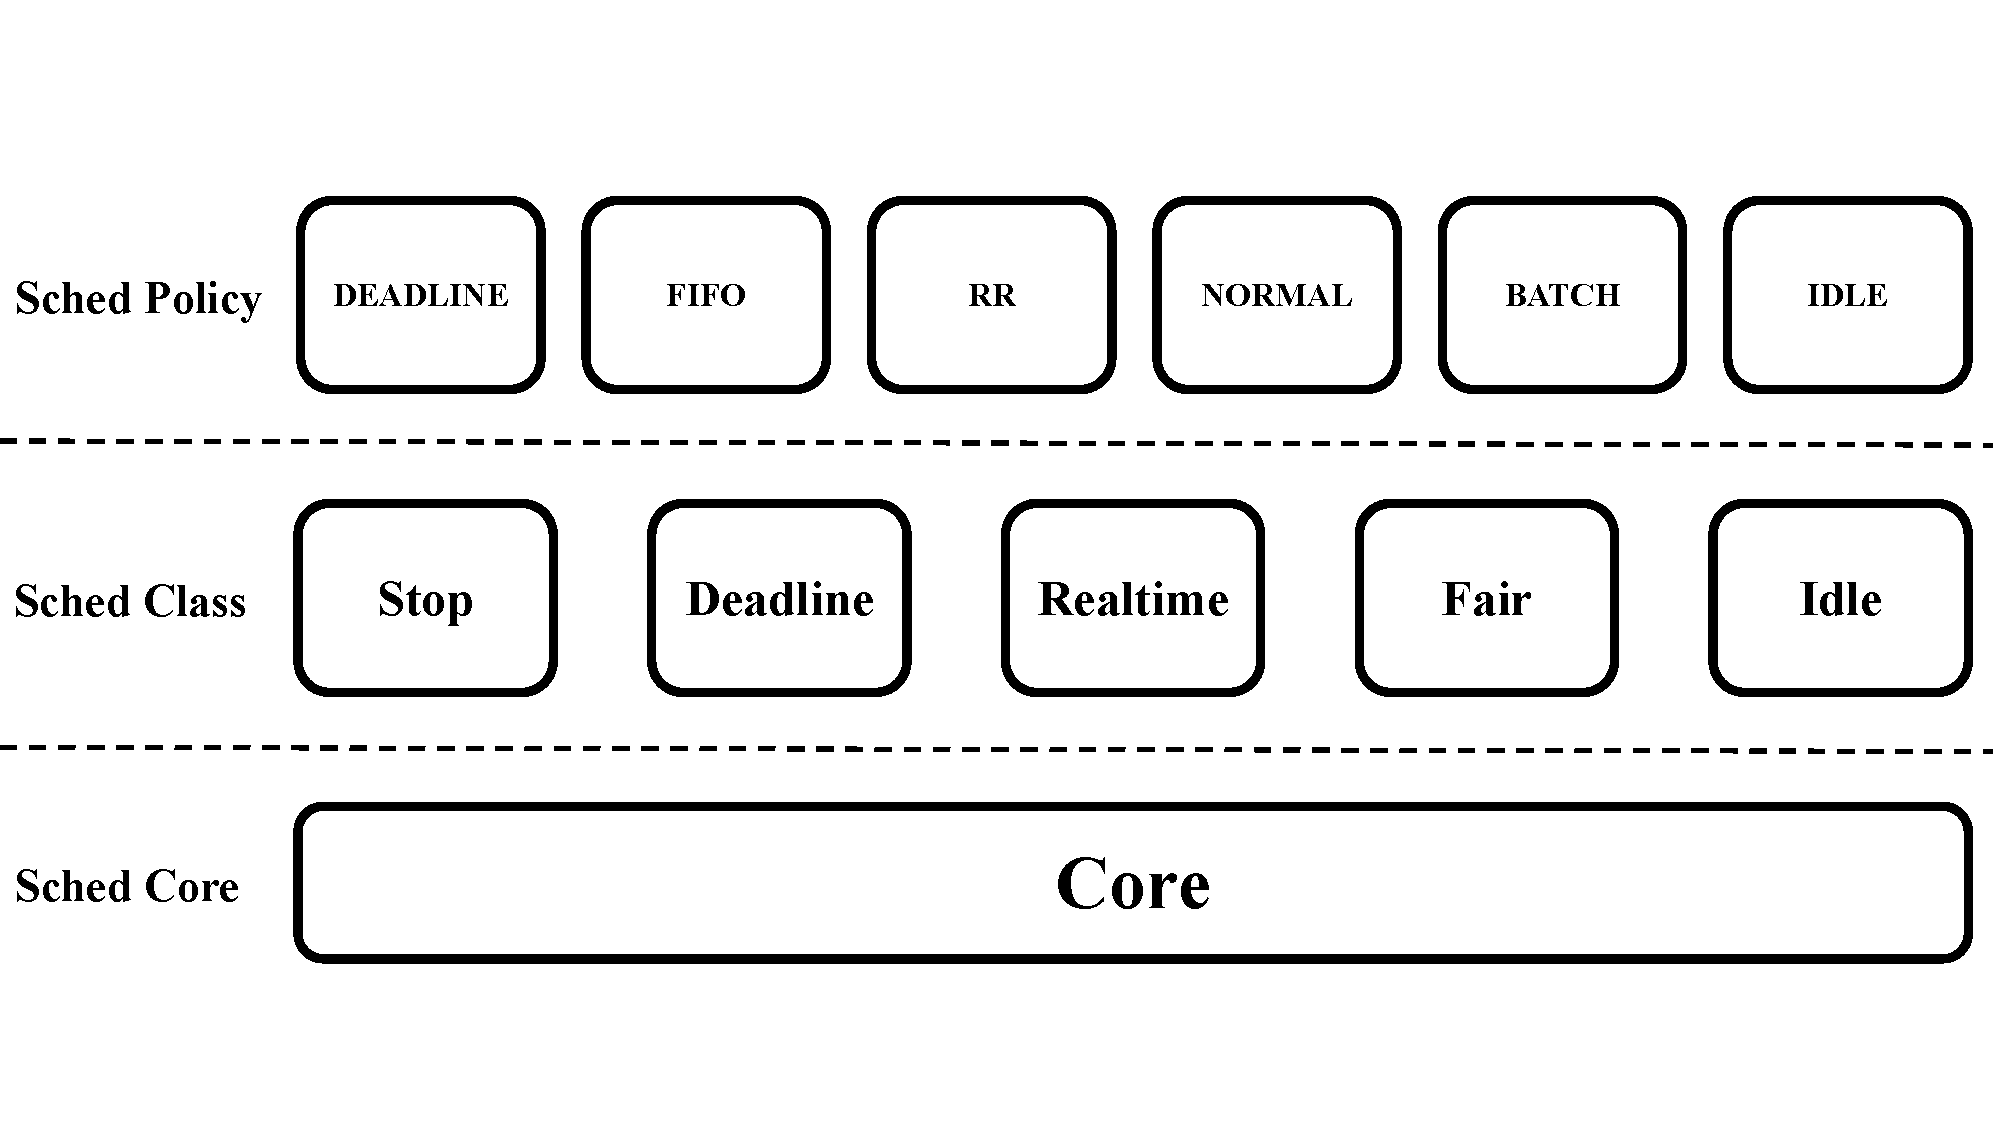
\includegraphics[width=0.7\textwidth]{sched_arch}
    \bicaption{\quad 调度子系统架构}{\quad Scheduling subsystem architecture}
    \label{fig:sched_arch}
\end{figure}

Core提供了最基本的调度框架,是所有调度机制的基本入口。Core调度可分为非抢占式调度与非抢占式两个部分,其中非抢占式调度部分来自于批处理调度,在这一场景中,任务依次执行直到退出。如图~\ref{fig:core_batch_sched}所示,Core调度器需要为新fork出来的任务选择合适的CPU并进行入队,而当任务exit或主动出让CPU之后,则需要重新进行出入队管理,并切换到下一个任务执行,这一过程即是调度循环,如图所示~\ref{fig:shcedule_loop},调度循环通常由中断或系统调用驱动,并在处理完毕到返回用户态之前的时候,通过判断标志位,来决定是否进入到调度循环的主逻辑。抢占调度部分则来自于时间片轮转调度,主要基于时钟中断机制来决策相同队列之上的任务切换,如图~\ref{fig:schedule_tick}所示,在时钟中断处理函数中,会触发Core中的task\_tick的执行,其中就会触发各个抢占式调度类的entity\_tick函数,来对当前任务的记账信息进行更新,当决策判断需要进行抢占时,就会通过Core提供的resched\_curr来设置抢占标记位,从而触发一次调度循环来进行任务抢占。

\begin{figure}[!htbp]
    \centering
    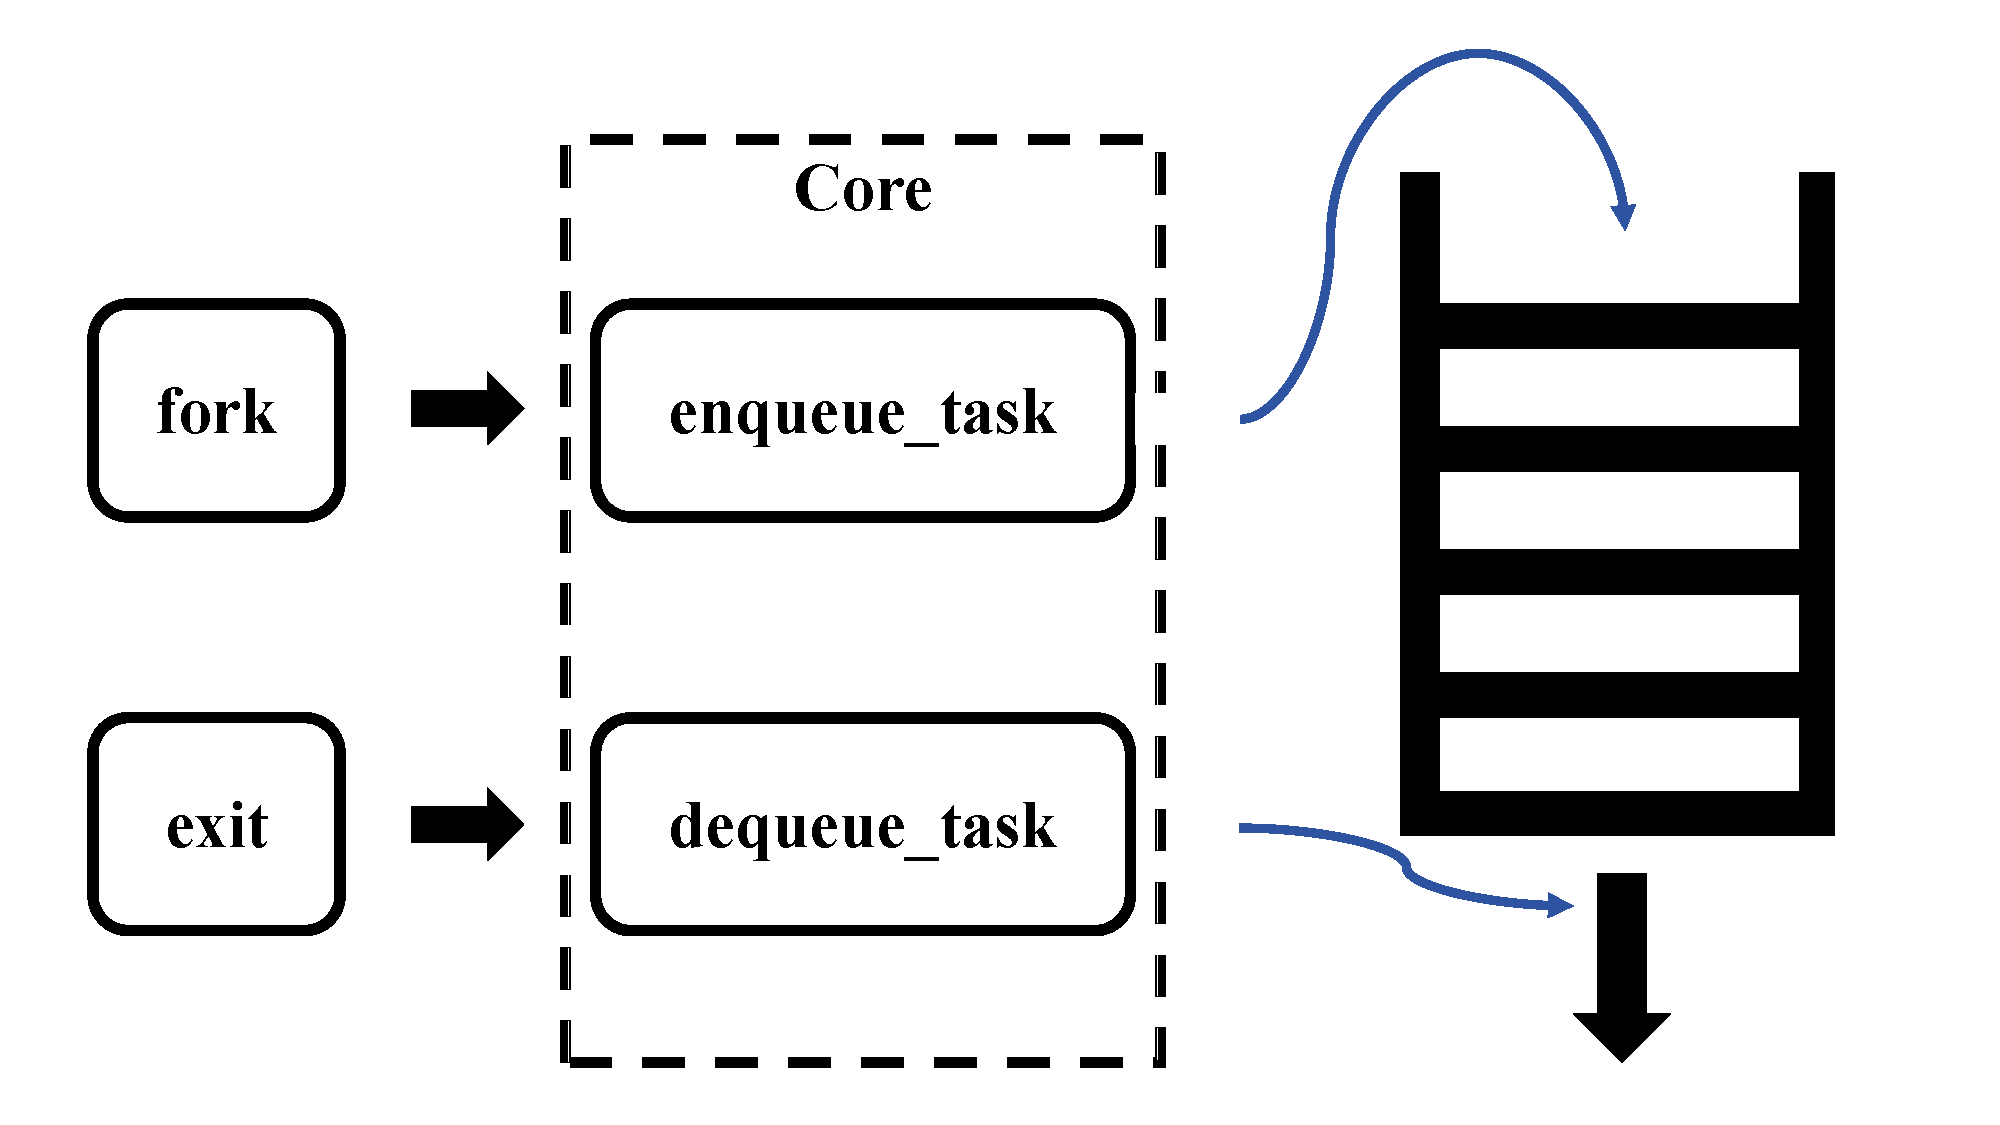
\includegraphics[width=0.7\textwidth]{core_batch_sched}
    \bicaption{\quad Core任务调度}{\quad Core scheduling tasks}
    \label{fig:core_batch_sched}
\end{figure}

调度类层基于Core所提供的基本框架进行设计。当前Linux中主要包含有Stop、Deadline、Realtime、Fair、Idle五大调度类\citep{scheduler},其中Stop调度类的实现最为简单,而其与Core调度的结合便是最早的批处理调度。Fair调度类最为复杂,使用到了大量如红黑树的高级数据结构,并采用了较为复杂的启发式算法与记账逻辑,最终实现了以公平为目标的调度,而其优异的特性使得其一般作为Linux中任务的默认调度类。其余调度类同样以不同的目标进行设计,同时Linux为这些调度类设置了不同的优先级,如图所示~\ref{fig:sched_ext_priorty}, 在每个调度循环中,会从最优先的调度类开始遍历,并依次调度任务执行。

\begin{figure}[!htbp]
    \centering 
    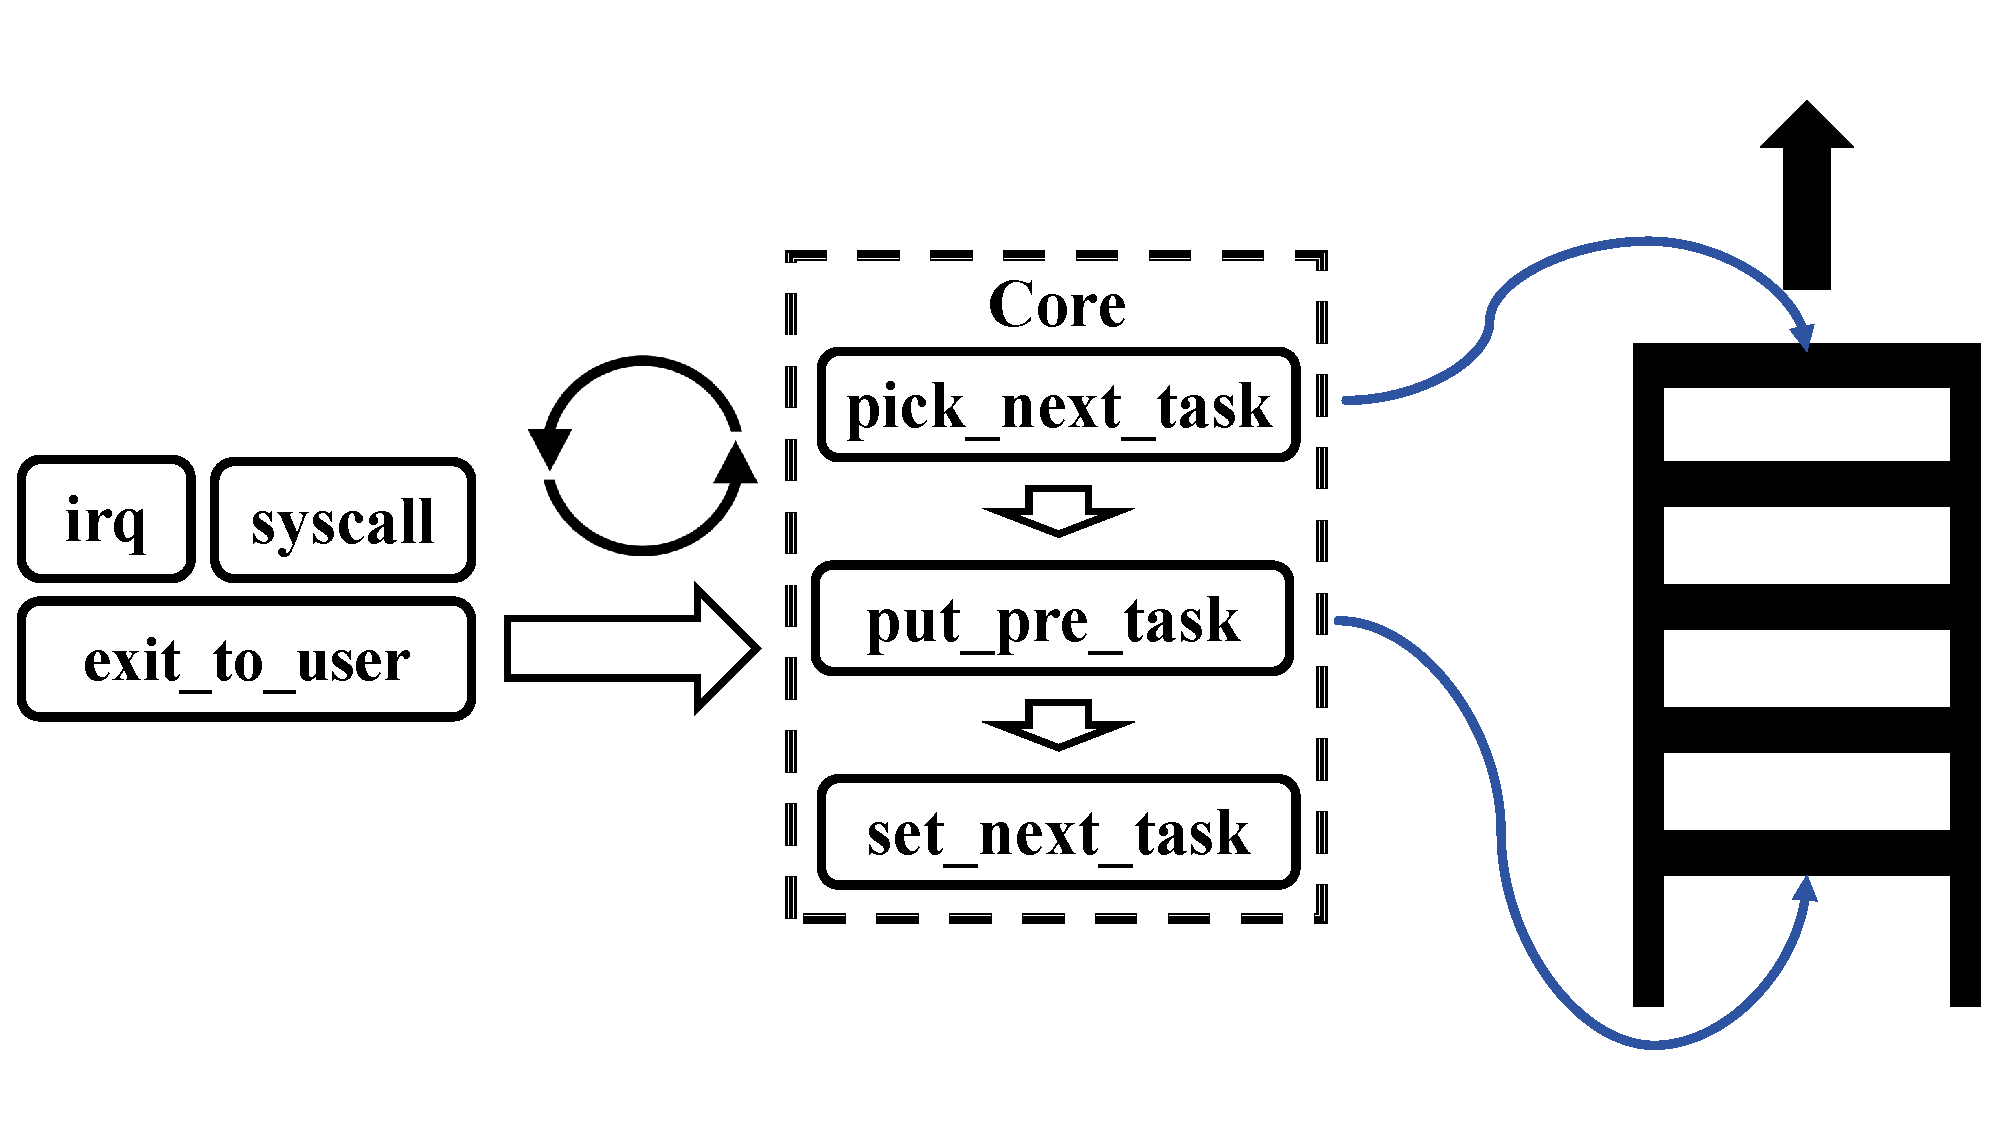
\includegraphics[width=0.7\textwidth]{shcedule_loop}
    \bicaption{\quad 调度循环}{\quad Schedule Loop}
    \label{fig:shcedule_loop}
\end{figure}

调度策略层围绕优先级机制实现,在各个调度类中的实现各不相同。在Realtime调度类中,优先级体现为多个调度队列,选取任务时会从最高优先级的任务队列开始,这保证了高优先级的任务被优先执行,而在同一个任务队列中,调度策略则区分了任务轮换的形式,如FIFO采用先来先执行的逻辑,而RR则通过时间片轮转依次执行任务。而在Fair调度类中,优先级机制的实现则完全不同,这与Fair调度类的算法实现相关,Fair调度类中会为每个任务维护一个vruntime,并在调度时选则vruntime最小的任务执行,优先级体现为vruntime积累的差异,即高优先级的任务积累vruntime的速度会更慢,而基于此Fair调度类提供了NORMAL与BATCH两种调度策略,实质对应为不同的优先级,来提供使用。

\begin{figure}[!htbp]
    \centering
    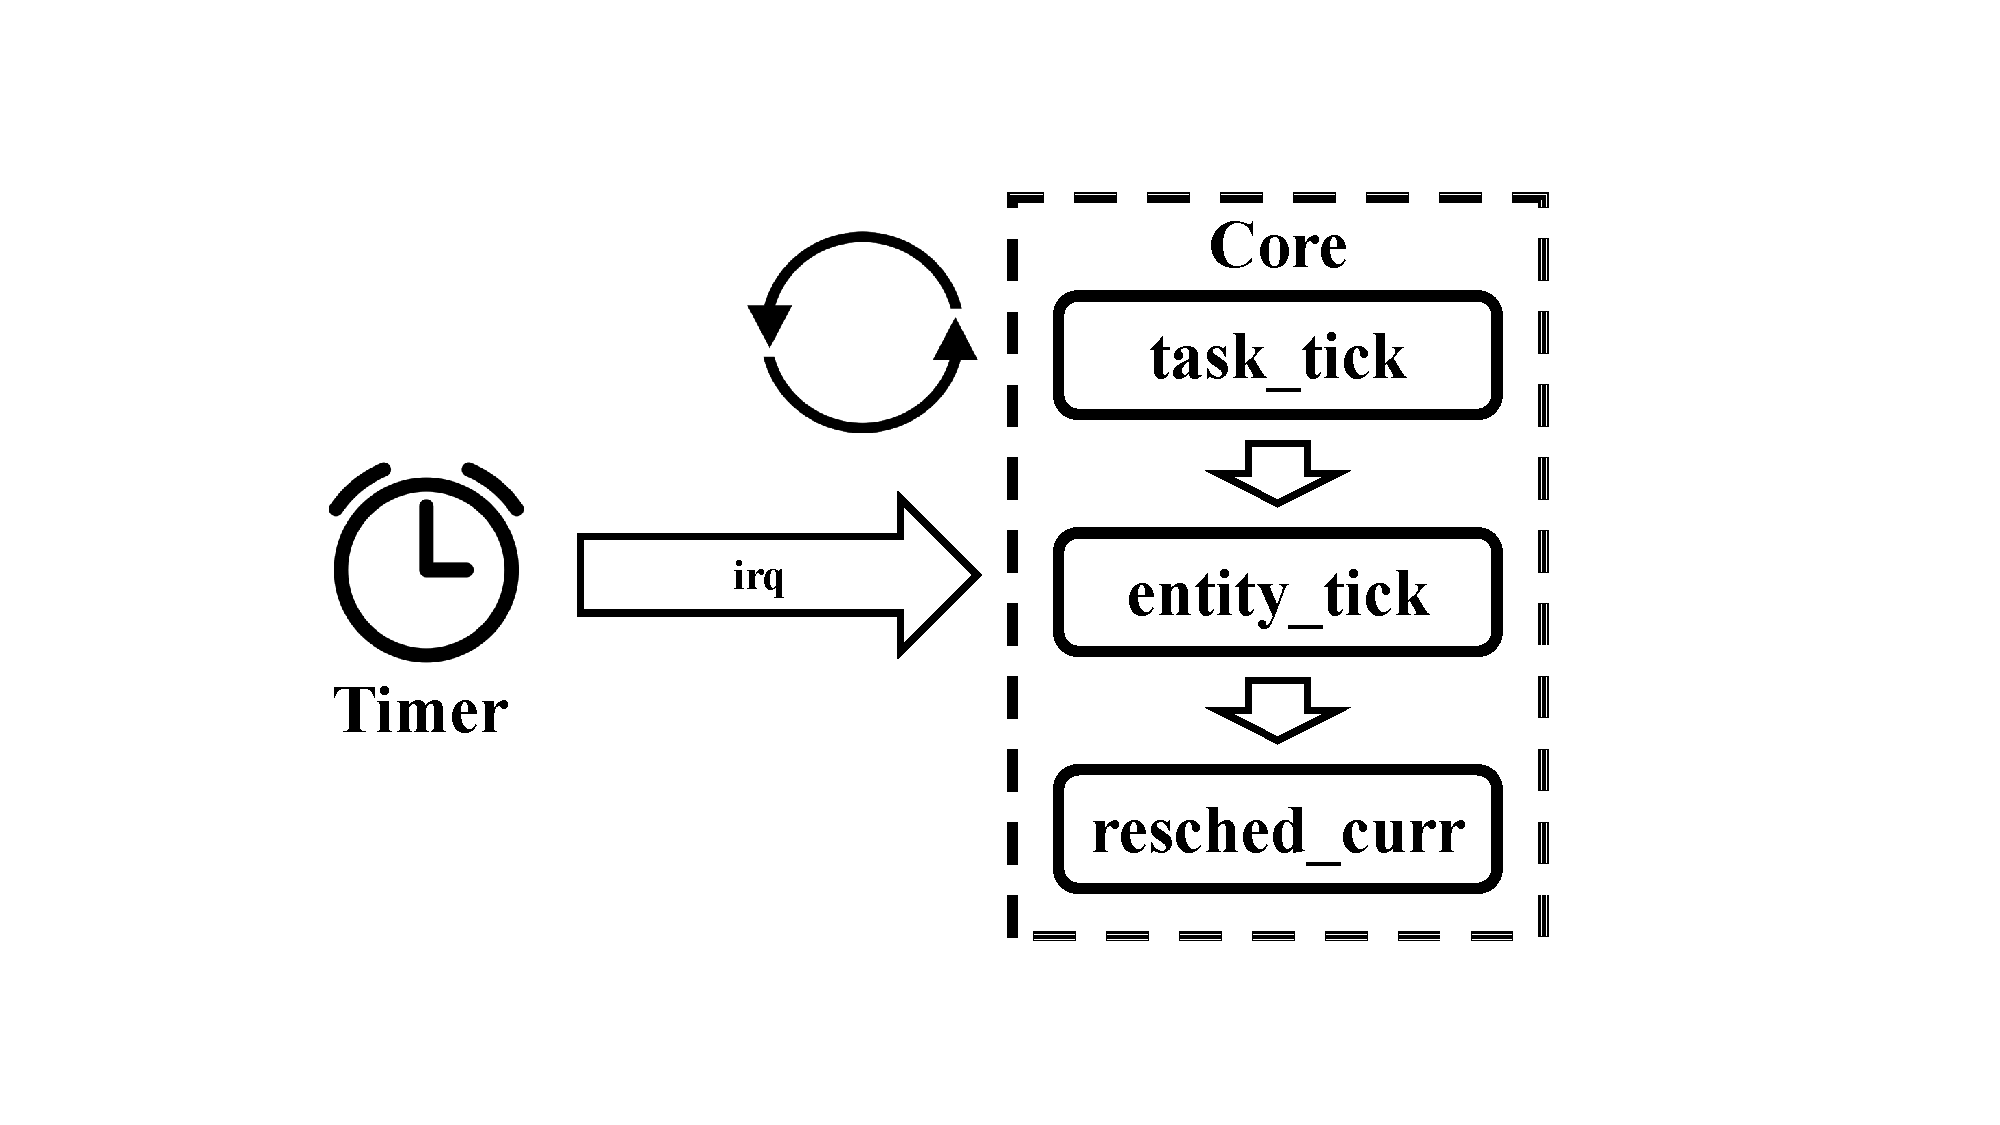
\includegraphics[width=0.7\textwidth]{schedule_tick}
    \bicaption{\quad 抢占调度时钟滴答}{\quad Schedule Tick}
    \label{fig:schedule_tick}
\end{figure}

调度器作为一种质量要求较高的系统组件,通常需要数十年的得带来进行完善\citep{agache2020firecracker},如EEVDF从算法提出到在Linux 6.6中被正式加入就经过29年,并且仍然在不断地被完善。同时调度器作为内核的核心机制,通常牵扯到许多内核中的复杂机制,如各种复杂的同步原语,同时内核环境也为开发者提出了诸多限制,因此在开发、测试与调试上都充满困难\citep{humphries2021ghost}。最后,即便调度器开发完毕,在部署上也存在很高的难度,由于内核无法在运行的状态中对调度器进行修改,因此调度器的部署通常都涉及到任务的迁移,而一旦调度出现错误,则很容易造成较大的损失。

\section{BPF技术}

% 定制内核的需求: 多样的硬件/多样的网络处理模式
% 内核模块: 灵活性高,但不安全,容易引发内核crash风险
% BPF在网络子系统引入,自定义网络包的处理流程
% 逐渐拓展到各个子系统中,但由于内核的审慎地设计,其他子系统中通常用来进行只读操作,如进行监测

eBPF(Extended Berkeley Packet Filter)是Linux内核中的一个轻量级、快速的64位的类RISC虚拟机\citep{sharaf2022extended}。当前eBPF当前已经成为在Linux内核运行时执行不可信的、由用户定义的专用代码的最佳实践与事实标准。其强大的性能、可移植性、灵活性与安全性得到了工业界和学术界的认可,并被广泛地用于更多的领域。

eBPF的前身是BPF(Berkeley Packet Filter),最早由McCanne和Jacobson设计并提出\citep{mccanne1993bsd},起初BPF如其名称所示,用于在Linux网络子系统中对网络包进行灵活处理,而因其本身优异的设计,被Linux内核社区的贡献者扩展到内核的各个子系统中,来对内核功能进行定制化,为了与旧BPF技术进行区分,内核社区将早期的BPF技术成为cBPF(Classic Berkeley Packet Filter),而BPF和eBPF均指代最新的BPF技术,本文在后续说明中也采用这种做法。

BPF本身是一种指令集,最初设计时考虑到安全性与易用性,允许开发者使用C语言的子集进行编写,并能作为一种编译器后端指令集,由GCC等常用编译器编译为字节码\citep{ebpfguidence}。BPF采用字节码的处于两种原因,其一是方便内核验证器对代码进行验证,其二则与Java思想类似,即利用字节码与语言虚拟机的组合提升可移植性。BPF虚拟机运行在内核中,Linux提供了相关的BPF系统调用来将字节码加载到内核中,并附加到代码中声明的钩子函数处,当对应函数触发时,内核态的BPF虚拟机就会执行附加的BPF字节码。整个过程中为了防止加载非法代码,内核首先会在加载BPF程序前对BPF字节码进行验证,判断是否符合在内核中执行的规范,如不允许死循环等,而在内核BPF虚拟机中执行时,会利用JIT技术将字节码映射到本机机器码,从而实现最佳的运行性能。

同作为对内核功能的扩展,BPF技术经常会与内核模块进行比较。相较于内核模块,BPF技术具有更高的安全性,BPF程序安全性体现在三个方面。首先不同于内核模块,BPF程序在编写时所有的对内核数据、地址的访问都需要通过BPF Helper函数来实现,同时,部分BPF Helper函数设计时就考虑到并发性,极大减少了不安全代码的数量。其次,BPF程序在加载时会被内核验证,同时由于运行在虚拟机中,也增强了安全性。最后,BPF程序所能执行的位置由内核提供,这样也大大缩小了危险代码的影响范围。

\begin{figure}[!htbp]
    \centering
    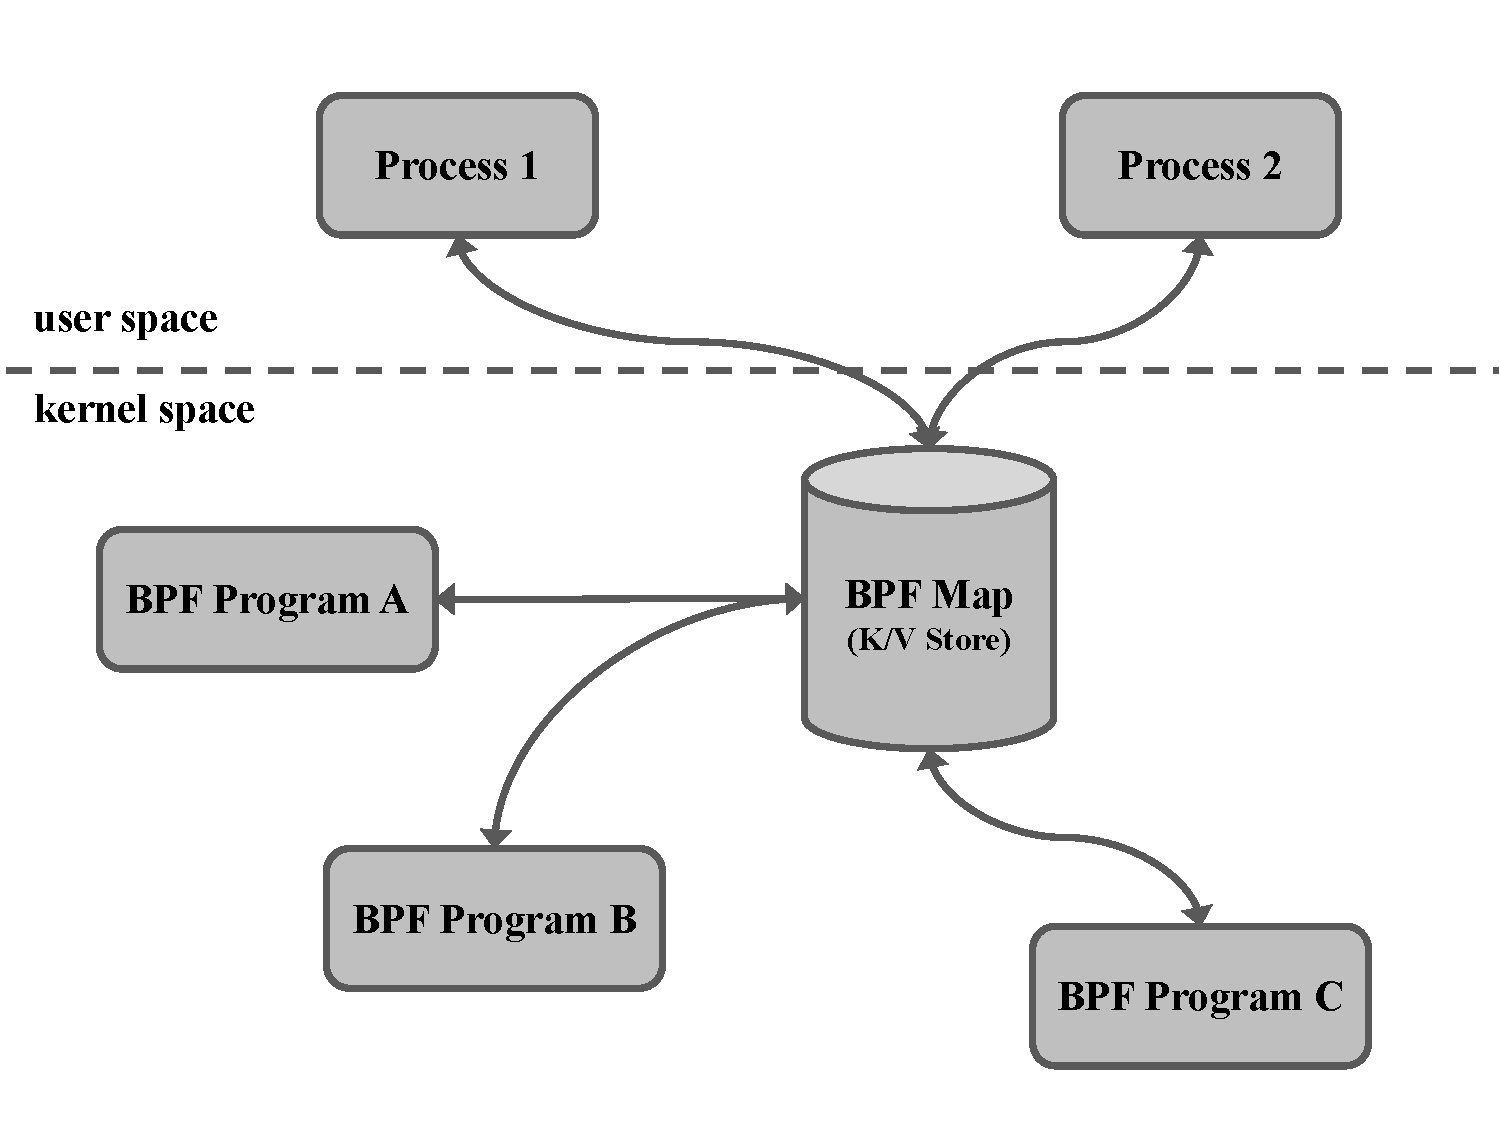
\includegraphics[width=0.6\textwidth]{bpf_user_kernel}
    \bicaption{\quad BPF中用户态与内核态的交互}{\quad Interaction between user mode and kernel mode in BPF}
    \label{fig:bpf_user_kernel}
\end{figure}

同时,BPF技术也具备高度的灵活性。这种灵活性体现在两个方面,首先对于用户态与内核态的交互,BPF技术运行由用户态的程序来加载BPF程序,由于BPF本身是字节码,因此能够借助libbpf等工具来对代码中的部分进行修改,这大大增强了BPF程序的灵活性。其次,如图~\ref{fig:bpf_user_kernel}所示,BPF技术允许通过BPF Map来实现用户态与内核的逻辑交互,一方面,内核态BPF程序所收集到的数据,能够借助BPF Map反馈给用户态程序进行处理,另一方面用户态程序也能通过BPF系统调用操作内BPF Map,对其中的内容进行读写,从而影响内核态BPF程序的行为。其次,BPF技术还允许BPF程序之间的交互,除上述通过BPF Map的交互外,如图~\ref{fig:bpf_to_bpf}所示,BPF程序还能够相互进行调用,从而进行数据传递,或通过多个BPF程序的调用,来突破内核对单个BPF函数的限制,从而实现更加复杂的代码逻辑。

\begin{figure}[!htbp]
    \centering
    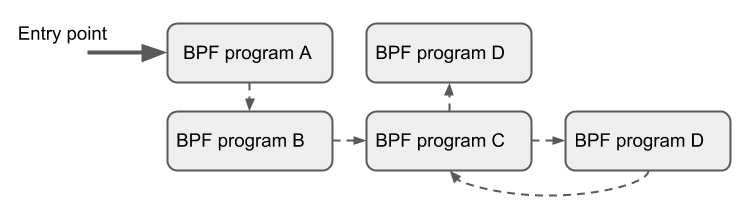
\includegraphics[width=0.7\textwidth]{bpf_to_bpf}
    \bicaption{\quad BPF程序之间的调用}{\quad Interaction between BPF programs}
    \label{fig:bpf_to_bpf}
\end{figure}

然而BPF技术也存在设计上的不足。由于在设计时首要考虑的是安全性,因此BPF程序在编写受到了种种限制,实际上,编写BPF程序所能使用的C语言子集是非图灵完备的,同时BPF程序在栈空间上也有严格的要求。这些限制都极大削弱了BPF程序的表达能力,使得其能够编写的逻辑十分有限。内核社区关注到这一点,并在近期的版本更新中逐步地减少对BPF程序的限制。

\section{可扩展调度类}

Sched Ext是一种可扩展的内核调度器设计\citep{schedext},由Meta以及内核社区的工程师共同设计实现,并已经在Meta的集群中运行与测试。Sched Ext最早提出于2022年,当前尚未合并入内核主线,但Meta与内核社区开发者十分活跃,Sched Ext当前仍然正在积极更新并持续地向内核社区提交Patch。

\begin{figure}[!htbp]
    \centering
    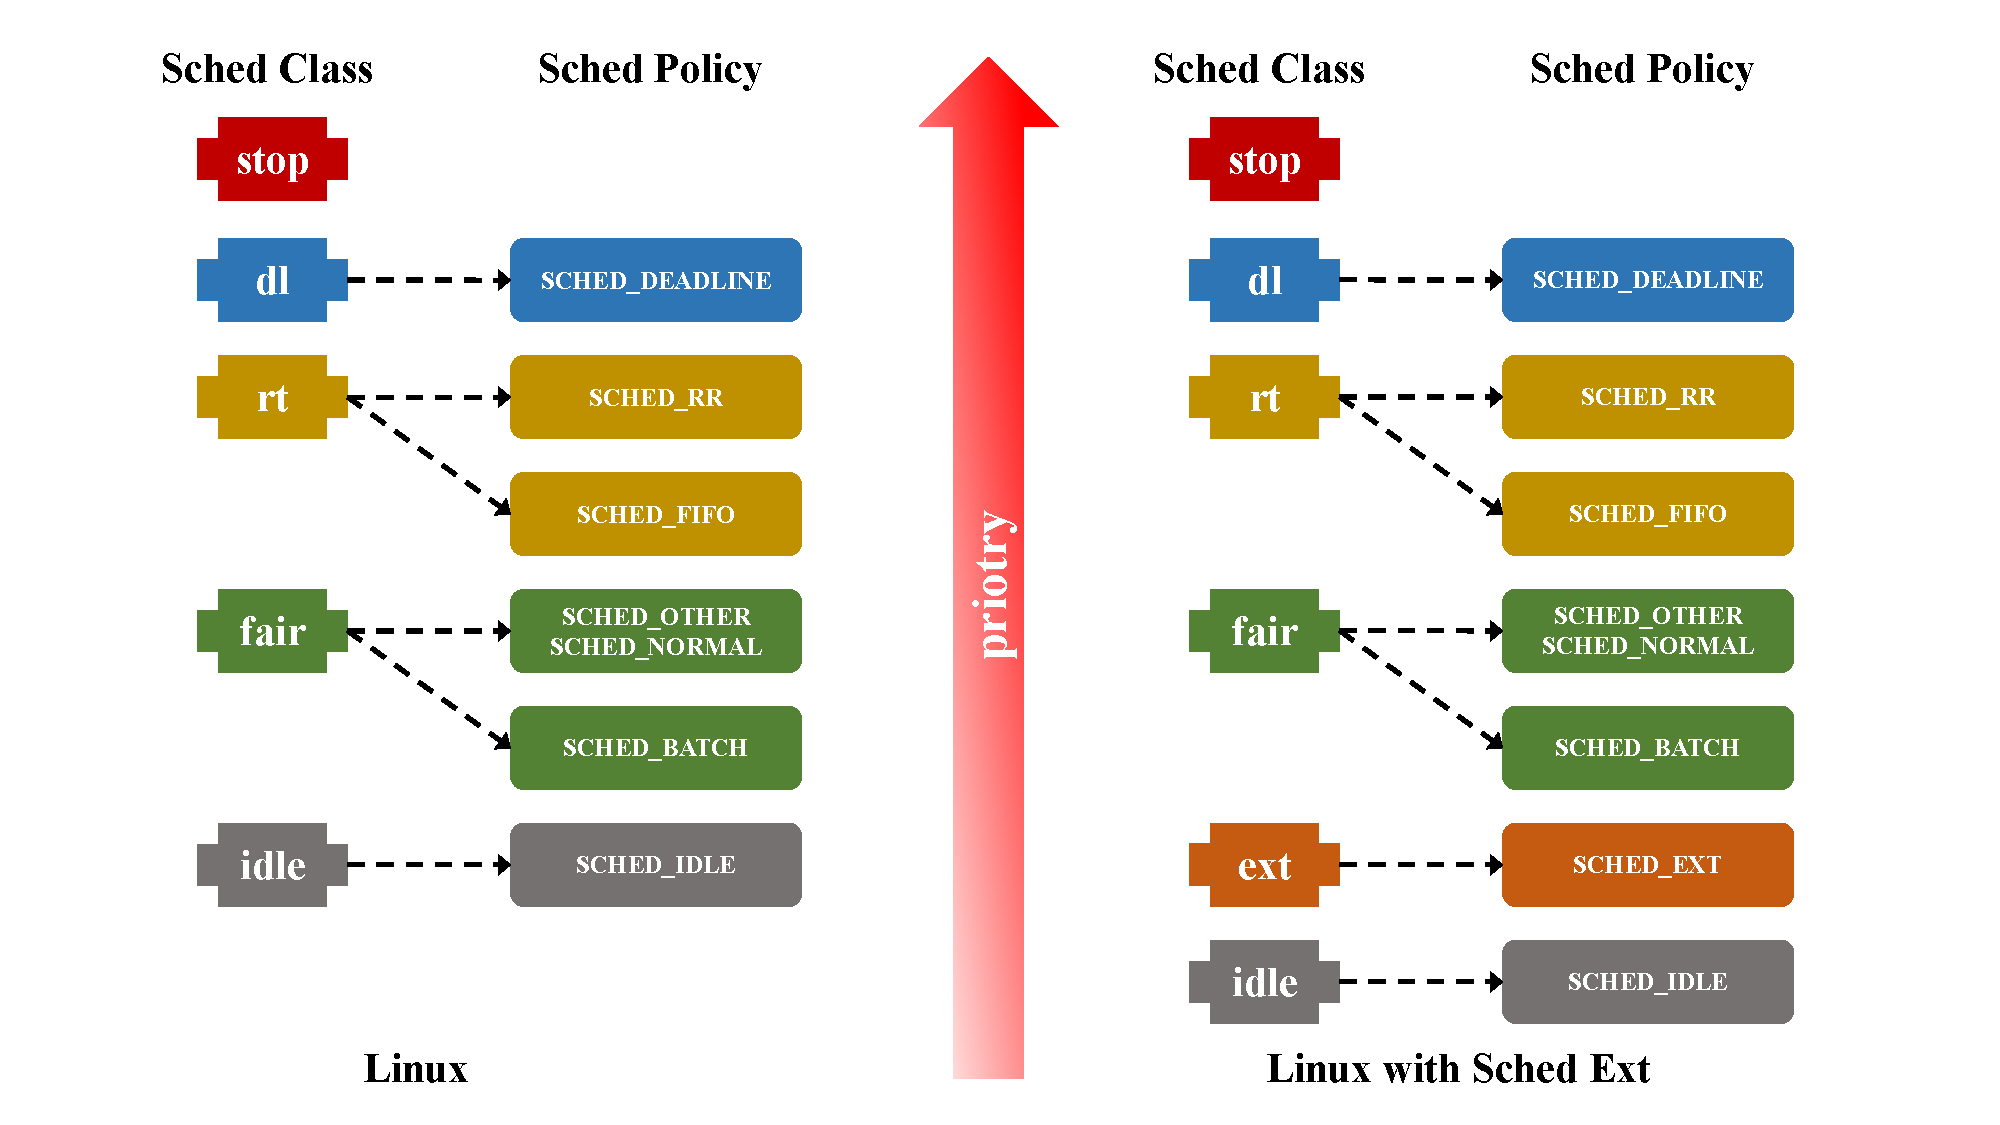
\includegraphics[width=1.0\textwidth]{sched_ext_priorty}
    \bicaption{\quad Sched Ext 调度优先级}{\quad Sched Ext Priorty}
    \label{fig:sched_ext_priorty}
\end{figure}

Sched Ext启发自ghOSt\citep{humphries2021ghost},考虑到内核调度器在开发与部署上的困难与当前数据中心对于定制调度器的需求的不匹配,因此期望设计一种插件化的调度器来提升内核调度器开发的灵活性。相较于ghOSt,Sched Ext在实现灵活调度的机制上存在两点差异,首先,Sched Ext设计之初就尽可能地保持与Linux现有调度机制的兼容性,如图~\ref{fig:sched_ext_priorty}所示的调度类优先级上,Sched EXt的默认优先级在Fair调度类与Idle调度类之间,同时Sched Ext调度类在没有BPF调度器加载时,默认将任务交给Fair调度类处理,通过以上两种处理,使得在使能Sched Ext时几乎不会对现有的调度机制产生影响。其次,Sched Ext调度的实现不局限于用户态,Sched Ext选择BPF来作为调度类的可扩展机制,通过增加BPF的特性,如增加Helper函数,扩展Map类型等,来使得其能满足编写调度器的基本要求,这样的设计使得一方面,开发者可以利用BPF的表达能力在内核态定制调度机制,另一方面也可以利用BPF程序与用户程序的互通性,在用户态设计调度器从而避开内核态编程的限制。

Sched Ext与其他调度类一致,实现了调度类所需要的全部方法。但与其他调度类不同的是,Sched Ext的调度过程需要与BPF Scheduler进行协作完成。而为让BPF Scheduler介入调度过程,Sched Ext调度类中首先定义了调度队列DSQ,通常每个CPU上都会有自己的Local DSQ,BPF Scheduler则可以拥有数个DSQ,task在不同的DSQ之间流转,而只有在CPU Local DSQ上时,才有被执行的机会,同时,Sched Ext围绕DSQ管理以及BPF与CPU的互动定义了一些列BPF Helper函数,这些Helper函数支持BPF Scheduler完成整个调度过程:

1)scx_bpf_create_dsq: 定义一个DSQ(调度队列)来对task进行管理。DSQ是BPF Scheduler管理task的核心, BPF程序中可以保有不止一个DSQ,DSQ之间通过ID来进行区分,同时通过NUMA亲和性能够来保证访问DSQ内存的效率。

2)scx_bpf_dispatch、scx_bpf_dispatch_vtime:将task调度到DSQ中。调度逻辑中可通过ID来指定目标DSQ以及task的运行slice,其中slice可以设置为无限,此时task不会被同队列中的其他任务抢占,而由BPF程序来决策抢占的时机。调度的任务通常以FIFO的形式入队,Sched Ext也提供了基于vtime的类CFS队列,以满足不同的BPF调度器的设计需求。

4)scx_bpf_dispatch_nr_slots:查看CPU可调度的task槽数。允许BPF程序检查当前CPU上可承载的task余量,避免BPF Scheduler向目标CPU调度过多的任务。

5)scx_bpf_dispatch_cancel:撤销最近向CPU调度的一个task。当task的CPU亲和性发生变化时,BPF Scheduler原先调度的task就应当进行变化,而此Helper函数便于BPF Scheduler撤销先前的调度决策。

6)scx_bpf_consume:将BPF scheduler管理的task调度给CPU。Sched Ext中的task需要经过从BPF Scheduler的调度队列到CPU本地调度对队列的过程,这一过程的通过此Helper函数完成。

7)scx_bpf_kick_cpu:激活CPU的重调度。BPF程序能够通过此Helper函数唤醒一个idle CPU或者让繁忙的CPU进入调度循环中,其中为避免唤醒的时间过程,采用向中断队列添加延时任务的形式异步地设置唤醒任务,而在唤醒的过程主要通过Core中提供的resched_curr完成。

8)scx_bpf_pick_idle_cpu:找到一个空闲的CPU。根据不同的调度目标,调度器应当避免任务过度的集中于同一个CPU,BPF Scheduler可以通过此Helper函数找到一个空闲CPU,将task调度到此CPU上,并结合其他Helper函数来唤醒CPU。

Sched Ext中实现的基本逻辑中已经具备足够的调度功能,作为基准的来保证基本的调度功能。BPF实现的调度逻辑被定义为sched_ext_ops保存在调度类中,随后在Sched Ext的执行过程中,BPF实现的调度操作会在进行调度决策的关键路径中触发,与Sched Ext的基准代码协作进行调度决策。

1)select_cpu:为唤醒的task选择一个CPU。这一过程通常发送在SMP系统中,需要考虑任务的特性以及CPU的负载情况,选择的结果会影响到系统总体的性能,因此BPF所实现的逻辑不一定是最终的调度结果,实际的调度决策还会结合调度类本身的决策与BPF的决策。

2)enqueue:处理task的入队。调度类所管理的任务就绪时,会在入队的关键路径上触发BPF enqueue的执行,BPF中可将task通过Helper函数发送到DSQ中,并进行后续的管理。

3)dequeue:处理task的出队。当需要对task的调度属性,如优先级,进行修改时,便会触发task出队逻辑,此时BPF中可以自定义优先级的更改逻辑,从而实现自定义的优先级功能。

4)dispatch:处理task的调度。BPF可以通过创建DSQ来持有task,同时每个CPU也拥有自己的Local DSQ来保存要执行的任务,当CPU的Local DSQ为空时,就会触发BPF的任务调度,期望从BPF的DSQ中获取将要执行的任务。BPF可以一次性调度多个任务,从而增加调度的效率,而任务的选择则完全由BPF程序决定。

5)runnable、running、stopping、quiescent:追踪task的状态。task通常会在如下三种情况进入Runnable状态,首先是被唤醒时,如从等待IO的状态中恢复,其次是从其他CPU迁入时,以及从队列中暂移后恢复时,如修改task优先级时,这些情况通过flag进行区分,并触发runnable的执行,quiescent的触发与上述时机完全相反,其他函数则在更细致的时机触发以反映task的状态,其中running对应task将要在CPU上运行时,stopping对应task将要停止运行时。BPF通过这些函数来追踪task的状态变化,从而辅助进行自定义的调度过程。

6)yield:让出CPU资源。Linux提供了sched_yield系统调用,允许task主动放弃CPU资源,通常用于多线程中。sched_yield并不保证线程组中的其他线程立即执行,而是将决策交给调度器,Sched Ext中此决策过程可完全由BPF程序实现。

7)init_task、exit_task: 追踪task的创建与退出。调度类中每当有task新创建或退出时触发,BPF可追踪这些事件,从而能够在BPF Scheduler中为每个任务定义额外的信息用于后续的调度过程。

如图~\ref{fig:sched_ext_arch}所示,Sched Ext基于BPF的可编程设计提供了丰富的手段来定制化调度过程。首先最直接的就是通过BPF程序定制调度逻辑,,这种方式的好处就在于所有的调度过程仍然在内核中进行,因此不会有用户态与内核态频繁切换的开销,而开发者仅需要提交BPF程序。其次,开发者可以直接操作任务队列来控制调度过程,Sched Ext将调度中核心的任务队列暴漏了出来,并允许通过BPF Help函数直接操作任务队列,这使得在调度程序完全能够在用户态进行实现,同时Sched Ext还提供了基于C与Rust语言的库函数,方便了开发者进行调度器设计,这种方式虽然引入了地址空间切换的开销,但也极大增加了调度器设计的灵活性。

\begin{figure}[!htbp]
    \centering
    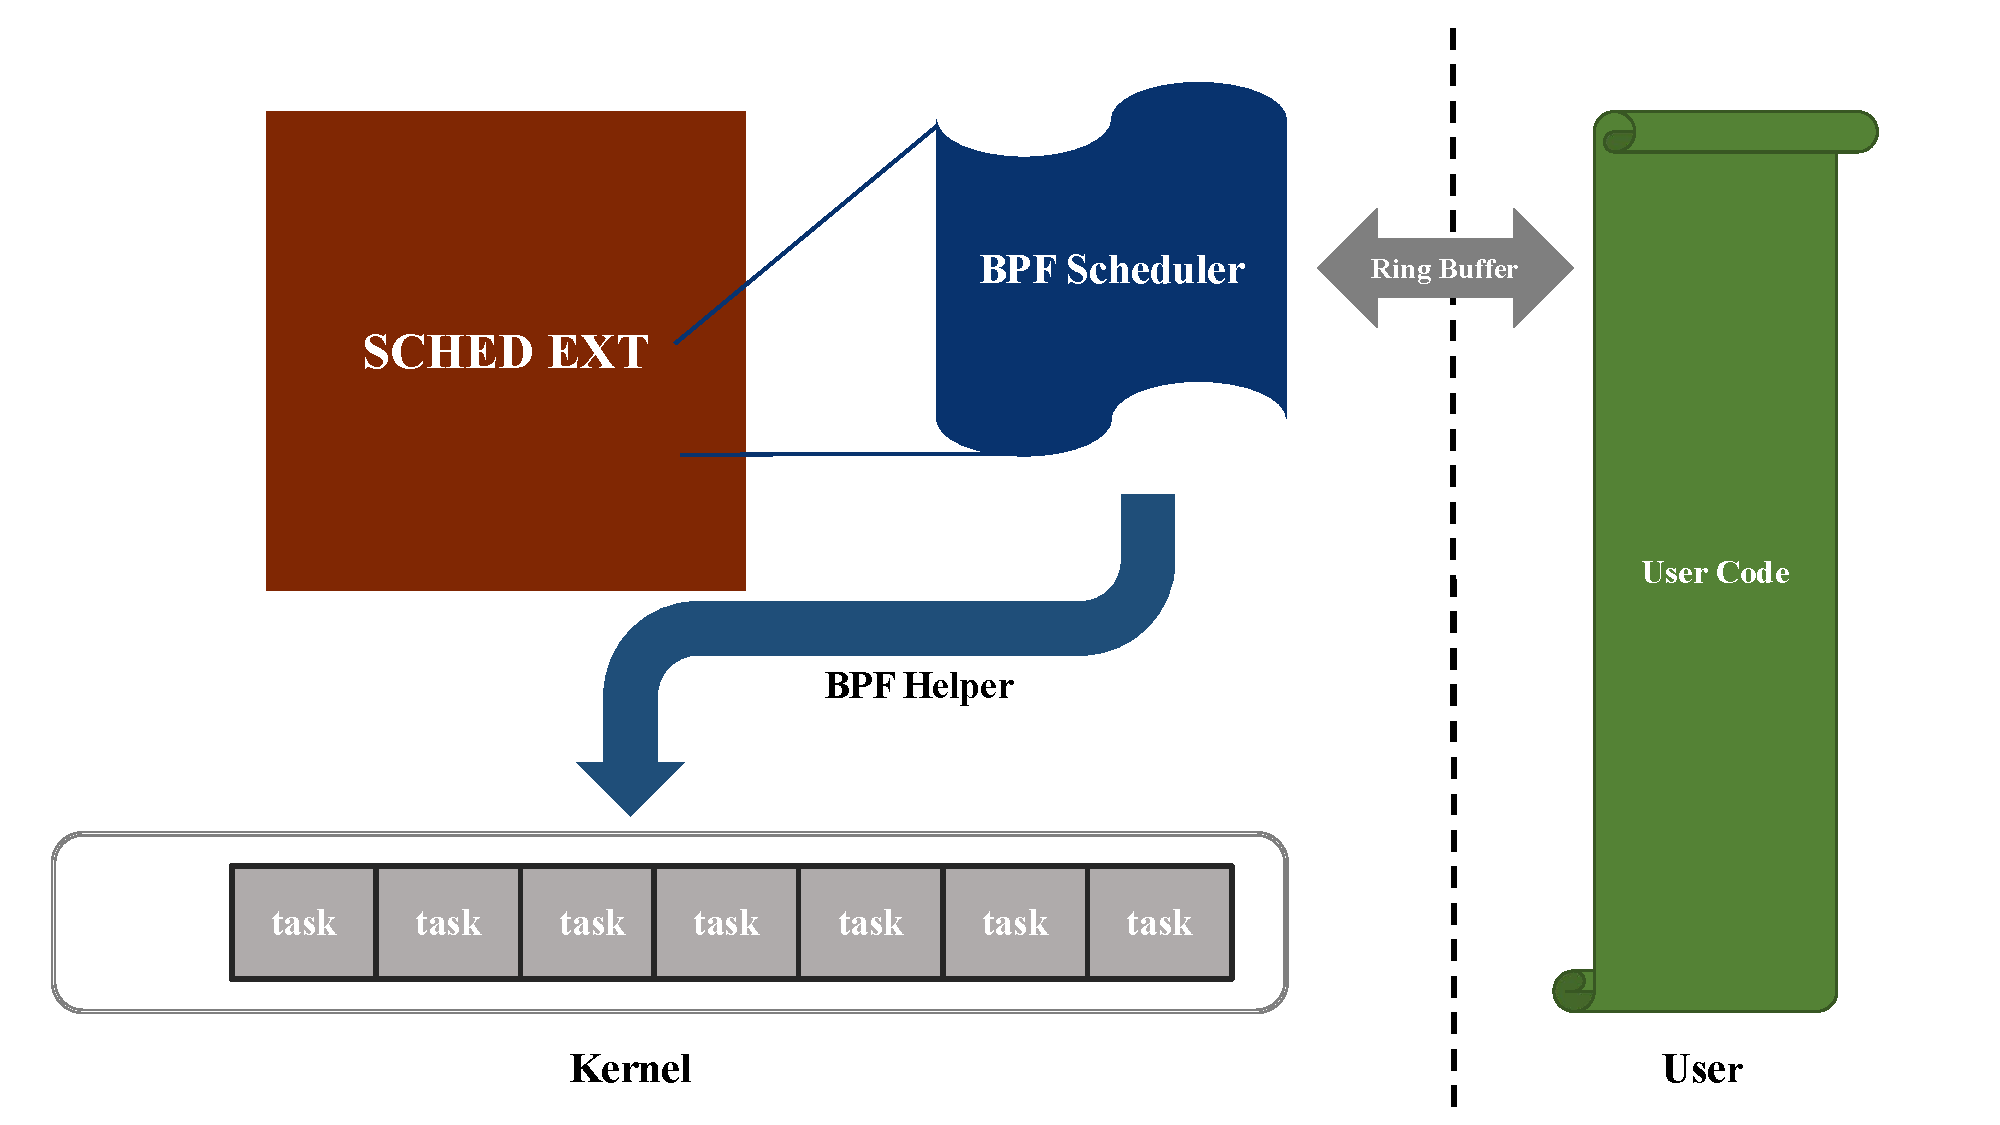
\includegraphics[width=0.7\textwidth]{sched_ext_arch}
    \bicaption{\quad Sched Ext架构}{\quad Sched Ext Arch}
    \label{fig:sched_ext_arch}
\end{figure}

默认情况下仅由Sched Ext类的任务会被BPF调度程序处理,而如果BPF调度程序尚未加载,Sched Ext调度类的任务仍然会交给Sched Normal进行处理,以避免任务得不到执行。同时,Sched Ext还允许通过特殊的BPF Helper函数,将SCHED NORMAL即以下的任务全部交给SCHED EXT进行处理,这种情况下,Sched Ext调度类就能够参与系统中核心的调度过程。

\section{沙箱技术}

% 系统级沙箱(虚拟机),容器级沙箱(进程)
% 安全性: 虚拟机 > 沙箱
% - 容器类沙箱缺乏调度机制的支持,而对调度机制的修改需要更安全的沙箱环境来限制风险的传播

沙箱技术是一种安全机制,用于隔离运行环境,以便在受限的环境中执行不受信任的程序或代码,并防止这些程序或代码对主机上其他任务造成影响或危害。沙箱是通过在受限的操作系统环境中执行软件来实现的,并对软件所能使用的资源,如CPU、内存、网络等进行限制。沙箱技术为在数据中心中安全地运行各种各样的应用提供了基础,而在数据中心中,常见的沙箱技术包括虚拟机技术与容器技术。

虚拟机技术是数据中心应用最广泛的沙箱技术,通常指通过软硬件的手段,在已运行的系统中模拟出一个硬件环境,并能够支持运行其他系统。虚拟机技术最早提出于\citep{bugnion1997disco}, 用于解决操作系统迭代速度与硬件更新速度不匹配的问题,而后

\section{本章小结}

本章主要介绍了eBPF技术以及Sched Ext可扩展内核调度机制。其中eBPF技术提供了一种集性能、灵活性于安全性于一体的扩展内核方式,利用eBPF技术能够方便地从内核中获取更多细致的数据,同时也能够在一些支持相对丰富的内核子系统中对内核功能进行定制。而Sched Ext提供了一种内核主线之外扩展内核调度的方式,其本身基于eBPF技术,因而能够利用到eBPF本身所具备的优势,同时其在调度子系统中展开了许多工作,使得通过eBPF程序定制调度逻辑成为可能,而其在设计上对于兼容性的考量,也方便了其在生产环境中的部署于测试。如上技术为本论文对应用进行细粒度监控,构造Control Zone与为不同混部场景设计不同的调度策略奠定了基础。